\documentclass{scrartcl}
\usepackage[utf8]{inputenc}
\usepackage{graphicx}%GRaphiken
\usepackage{tabularx}%Tabellen!
\usepackage{url}% Urls besser
\usepackage{textcomp}% Sonderzeichen
\usepackage{amsmath}%maths / equations
\usepackage{booktabs} % for cmidrule
\usepackage{todonotes}
\usepackage[
	left=3cm,
	right=2cm,
	top=1.5cm,
	bottom=1cm,
	includeheadfoot
	]{geometry}														% Satzspiegel
\usepackage[
	round,	%(defaultage in the main file and \input ) for round parentheses;
	%square,	% for square brackets;
	%curly,	% for curly braces;
	%angle,	% for angle brackets;
	colon,	% (default) to separate multiple citations with colons;
	%comma,	% to use commas as separaters;
	authoryear,% (default) for author-year citations;
	%numbers,	% for numerical citations;
	%super,	% for superscripted numerical citations, as in Nature;
	sort,		% orders multiple citations into the sequence in which they appear in the list of 				references;
	%sort&compress,    % as sort but in addition multiple numerical citations
                   % are compressed if possible (as 3-6, 15);
	%longnamesfirst,  % makes the first citation of any reference the equivalent of
                   % the starred variant (full author list) and subsequent citations
                   %normal (abbreviated list);
	%sectionbib,      % redefines \thebibliography to issue \section* instead of \chapter*;
                   % valid only for classes with a \chapter command;
                   % to be used with the chapterbib package;
	%nonamebreak,     % keeps all the authors names in a citation on one line;
                   %causes overfull hboxes but helps with some hyperref problems.
]{natbib}											    			% Literaturverzeichnis
\usepackage[pdfpagelabels,plainpages=false, pageanchor=false]{hyperref}	


%% andere Einstellungen
\linespread{1.5}% 1.5 Zeilenabstand			
\graphicspath{{fig/}}                     % path to graphics


%% ----------------------------------------------------------------------------
\title{Ecotoxicology is not normal.}
\subtitle{How the use of proper statistical models can increase statistical power in ecotoxicological experiments.}
\author{Eduard Szöcs, Ralf B. Schäfer}
\date{\today}



%% ----------------------------------------------------------------------------
\begin{document}
\maketitle

%% --------------------------------
\section*{Abstract}
Ecotoxicologist are often confronted with non-normally distributed data.
To achieve the assumptions of normality and heteroscedasticity is has been a standard procedure to either transform the data or use non-parametric methods if this fails.
Here, we argue that using appropriate models, namely Generalised Linear Models (GLM), can enhance statistical power.

We present examples of ecotoxicological studies illustrating the differences and advantages of GLM.
Using simulations of two common data types (counts and discrete proportions), we show that GLMs provide a gain in statistical power compared to analysis of transformed data or using non-parametric methods.
Moreover, GLMs provide a gain in interpretability of results.

GLMs should become a standard method in ecotoxicology to analyse inherently non-normally distributed data.




%% --------------------------------
\section{Introduction}
\label{sec:intro}
Ecotoxicologists perform various kinds of experiments yielding different types of data.
Examples are: animal counts in mesocosm experiments (positive, integer-valued data), proportions of surviving animals (data bonded between 0 and 1, continuous) or biomass in growth experiments (positive, continuous data).
These data are typically not normally distributed. 
Nevertheless, they are usually analysed using methods assuming a normal distribution and variance homogeneity \citep{wang_making_2011}. 
To meet these assumptions, data are usually transformed.
For example, ecotoxicological textbooks \citep{newman_quantitative_2012} and guidelines \citep{epa_methods_2002,oecd_current_2006} advise that survival data can be transformed using an arcsine square root transformation. 
For count data from mesocosm experiments a log(Ay + C) transformation is usually applied, where the constants A and C are either chosen arbitrarily or following general recommendations. 
For example, \citet{van_den_brink_impact_2000} suggest to set the term Ay to be 2 for the lowest abundance value (y) greater than zero and C to 1. 
Moreover, other transformations like the square root or fourth root are commonly applied in community ecology.
Note that there has been little evaluation and advice for practitioners, which transformations to use.
If the transformed data still do not meet the assumptions (i. e. normality and variance homogeneity), non-parametric tests are usually applied \citep{wang_making_2011}.

Generalized linear models (GLM) provide a method to analyse such non-normally distributed data \citep{nelder_generalized_1972}.
GLMs can handle various types of data distributions, e.g. Poisson or negative binomial (for count data) or binomial (for proportions); the normal distribution being a special case of GLMs.
Despite GLMs being available more than 40 years, ecotoxicologists do not regularly make use of them.

Recent studies concluded that data transformations should be avoided and GLMs be used as they have better statistical properties \citep{ohara_not_2010, warton_arcsine_2011}. 
Low sample sizes are common in ecotoxicological studies \citep{sanderson_pesticide_2002, szocs_analysing_2015} and lead to low power in statistical hypothesis testing, on which many ecotoxiological approaches (e.g. risk assessment for pesticides) rely. 
Differences between statistical methods may be apparent especially at such low sample sizes.

We explore how GLMs may enhance inference in ecotoxicological studies. 
We compared three types of statistical methods (transformation and normality assumption, GLM, non-parametric tests) using simulations and demonstrate on example data sets how conclusions can be influenced by the choice of statistical method.

\todo{LOEC rein}
\todo{Interpretation rein}


%% --------------------------------
\section{Methods}
\label{sec:methods}
\todo{Methods einleiten}
\subsection{Models for count data}
\subsubsection{Linear model for transformed data}
To meet the assumptions of the standard linear model count data usually needs to be transformed. 
We followed the recommendations of \citet{van_den_brink_impact_2000} and used a log(Ay + 1) transformation (eqn. \ref{eqn:trans}):

\begin{align}
  y^T_i & = log(Ay_i + 1) \label{eqn:trans} \\
  A & = 2~/~min(y)~~~\text{, for}~ y > 0 \nonumber
\end{align}

, where $y_i$ is the measured abundance and $y_i^T$ the transformed abundance. 

Then we fitted the linear model to the transformed abundances:

\begin{align}
  y_i^T &\sim N(\mu_i, \sigma^2) \nonumber \\
  y_i^T &= \alpha + \beta x_i \label{eqn:normal} \\
  var(y_i^T) &= \sigma^2 \nonumber
\end{align}

This model assumes a normal distributed response with constant variance ($\sigma^2$).
Note, that we parametrised the model as contrast ($\beta x_i$) to the control group ($\alpha$) so that parameters ($\beta$) are directly interpretable as changes from the control group (eqn. \ref{eqn:normal}).


\subsubsection{Generalized Linear Models}
Instead of transforming the response variable the counts could be directly modelled by a Poisson distribution:

\begin{align}
  y_i &\sim P(\lambda_i) \nonumber \\
  log(\lambda_i) &= \mu_i \label{eqn:pois} \\
  \mu_i &= \alpha + \beta x_i \nonumber \\
  var(y_i) &= \lambda_i \nonumber
\end{align}

Again, this model was parametrised as contrast to the control group. 
The response variable is linked to the predictors via a log-function to avoid negative fitted values (eqn. \ref{eqn:pois}). 
The Poisson distribution assumes that mean and variance are equal - an assumption that is rarely met with ecological data which is typically characterized by greater variance (overdispersion).
To overcome this problem a quasi-Poisson distribution could be used which introduces an additional overdispersion parameter ($\Theta$) (eqn. \ref{eqn:quasi}).

\begin{align}
  y_i &\sim P(\lambda_i, \Theta) \label{eqn:quasi} \\
  % log~\lambda &= \mu \label{eqn:quasi} \\
  % \mu &= \alpha + \beta X \nonumber \\
  var(y_i) &= \Theta \lambda_i  \nonumber
\end{align}

Another possibility to deal with overdispersion is to use a negative binomial distribution which also introduces an additional parameter (eqn. \ref{eqn:negbin}).

\begin{align}
  y_i &\sim NB(\lambda, \kappa) \label{eqn:negbin}  \\
  % log~\lambda &= \mu \label{eqn:negbin} \\
  % \mu &= \alpha + \beta X \nonumber \\
  var(y_i) &= \lambda_i + \kappa \lambda_i^2 \nonumber
\end{align}

In both cases the parametrisation and link function is equal to the Poisson GLM (eqn. \ref{eqn:pois}).
Note, that the quasi-Poisson model assumes a linear mean-variance relationship (eqn. \ref{eqn:quasi}), whereas the negative binomial model assumes a quadratic relationship (eqn. \ref{eqn:negbin}).
The above described models are most commonly used in ecology \citep{ver_hoef_quasi-poisson_2007}, although other distributions for count data are possible, like the negative binomial model with a linear mean-variance relationship (also known as NB1) or the poisson inverse gaussian model \citep{hilbe_modeling_2014}.


\subsection{Models for binomial data}
\subsubsection{Linear model for transformed data}
To accommodate the assumption for the standard linear model a special arcsine square root transformation (eqn. \ref{eqn:arcsine}) is suggested for such  data \citep{epa_methods_2002,newman_quantitative_2012}:

\begin{align}
  y_i^T = 
  \begin{cases}  
    arcsin(1) - arcsin(\sqrt{\frac{1}{4n}}) & \text{, if}\ y_i = 1 \\
    arcsin(\sqrt{\frac{1}{4n}}) & \text{, if}\ y_i = 0  \\
    arcsin(\sqrt{y_i}) & \text{, otherwise}
  \end{cases} \label{eqn:arcsine}
\end{align}

, where $y_i^T$ are the transformed proportions and n is the number of exposed animals per treatment ($n = 4 \cdot 10=40$).
The transformed proportions are then analysed using the standard linear model (eqn. \ref{eqn:normal}).
Note, that the parameters of the linear model are not directly interpretable due to transformation.


\subsubsection{Generalized Linear Models}
Data of type \emph{x out of N} can be modelled by a binomial distribution with parameters N and $\pi$:

\begin{align}
  y_i &\sim Bin(N, \pi_i) \nonumber \\
  logit~(\pi_i) &= \alpha + \beta x_i \label{eqn:bin} \\
  var(y_i) &=  \pi_i (1 - \pi_i) / N \nonumber
\end{align}

, where N = number of exposed animals and $\pi$ is the probability of survival.
The variance of the binomial distribution is a quadratic function of the mean (eqn. \ref{eqn:bin}).
The parameters $\beta$ of this model are directly interpretable as changes in log odds compared to the control group.


\subsection{Inference on models}
\todo{Überarbeiten}
On this data set, we could test different hypotheses like (i) if there is any effect of the treatment or (ii) test single parameters (treatments) to determine the LOEC.
Following general recommendations \citep{bolker_generalized_2009}, we used F-tests for the normal and quasi-Poisson models and Likelihood-Ratio (LR) tests for Poisson and negative binomial models to test if there is any treatment related effect.
To assess the LOEC we used Dunnett contrasts with one-sided Wald t tests (normal and quasi-Poisson models) and one-sided Wald Z tests (Poisson and negative binomial models).


\subsection{Case studies}
A full exemplary analysis of this data using R \citep{r_core_team_r:_2014} can be found in Supplement 2. \todo{wohin damit?}

\subsubsection{Count data}
\citet{brock_minimum_2015} presents a typical example of data from mesocosm studies.
The data are mayfly larvae counts on artificial substrate samplers were at one sampling date (Figure \ref{fig:example}). 
A total of 18 mesocosm have been sampled from 6 treatments (Control (n = 4), 0.1, 0.3, 1, 3 mg/L (n = 3) and 10 mg/L (n = 2)).


\subsubsection{Binomial data}
\citet{weber_short-term_1989} studied fathead minnow (\textit{Pimephales promelas}) larval survival data after sodium pentachlorophenol (NaPCP) exposure.
This data set is available in \citet{newman_quantitative_2012} and \citet{epa_methods_2002}.
Four replicates of ten fish were exposed to each of six six NaPCP concentrations (0, 32, 64, 128, 256, 512 \textmu g/L) and the proportion of total number alive at the end were reported. 


\subsection{Simulations}
\subsubsection{Count data}
We simulated count data that mimics count data encountered in mesocosm experiments with five treatments (T1 - T5) and one control group (C).
Counts were drawn from a negative binomial distribution with slight over dispersion (dispersion parameter for all treatments: $\kappa = 0.25$).
We simulated data sets with different number of replicates (N = \{3, 6, 9\}) and different abundances in control treatments ($\mu_\text{\tiny C}$ = \{2, 4, 8, 16, 32, 64, 128\}). 
For power estimation mean abundance in treatments T2 - T5 was reduced to half of control and T1 ($\mu_\text{\tiny T2}~=~...~=~\mu_\text{\tiny T5}~=~0.5~\mu_\text{\tiny C} = 0.5~\mu_\text{\tiny T1}$), resulting to a theoretical LOEC at T2.
Mean abundance was kept equal between all groups in Type I error simulations.

We generated 100 data sets for each combination of N and $\mu_\text{\tiny C}$. 
We fitted a linear model after log (Ax + 1) transformation ($LM$), negative binomial GLM ($GLM_{nb}$) and quasi-Poisson GLM ($GLM_{qp}$) to these datasets. 
We tested a general treatment effect using F tests ($LM$ and $GLM_{qp}$) and LR tests ($GLM_{nb}$). Additionally, we applied parametric bootstrap (500 bootstrap samples; \citet{faraway_extending_2006}) to assess the LR in the negative binomial model ($GLM_{pb}$) and used a Kruskal-Wallis test on untransformed data as a non-parametric method.
To assess the performance in detecting the LOEC (T2 in our simulation design) we used a one-sided Dunnett test for all models and a one-sided pairwise Wilcoxon test as a non-parametric method.
\todo{rerun!}


\subsubsection{Binomial data}
We simulated data from a design as described in the motivating example, with 5 treated (T1 - T5) and a control group (C). 
Proportions were drawn from a Bin(10, $\pi$) distribution, with varying probability of survival ($\pi$ = \{0.60, 0.65, 0.70, 0.75, 0.80, 0.85, 0.90, 0.95\}) and varying number of replicates (N = \{3, 6, 9\}).
For Type I error estimation, $\pi$ was held constant between groups.
For power estimation $\pi$ in C and T1 was fixed at 0.95 and was set to values between 0.6 and 0.95 for the treatments T2 - T5. 
 
We simulated 250 data sets for each combination and analysed them using the linear model after arcsine transformation (LM), binomial GLM (GLM) and Kruskal-Wallis test.
Moreover, we compared the methods' ability to determine the LOEC (T2 in our simulation design) by comparing inferences on model parameters and a pairwise Wilcoxon test. 







%% --------------------------------
\section{Rest}


\begin{figure}
  \centering
  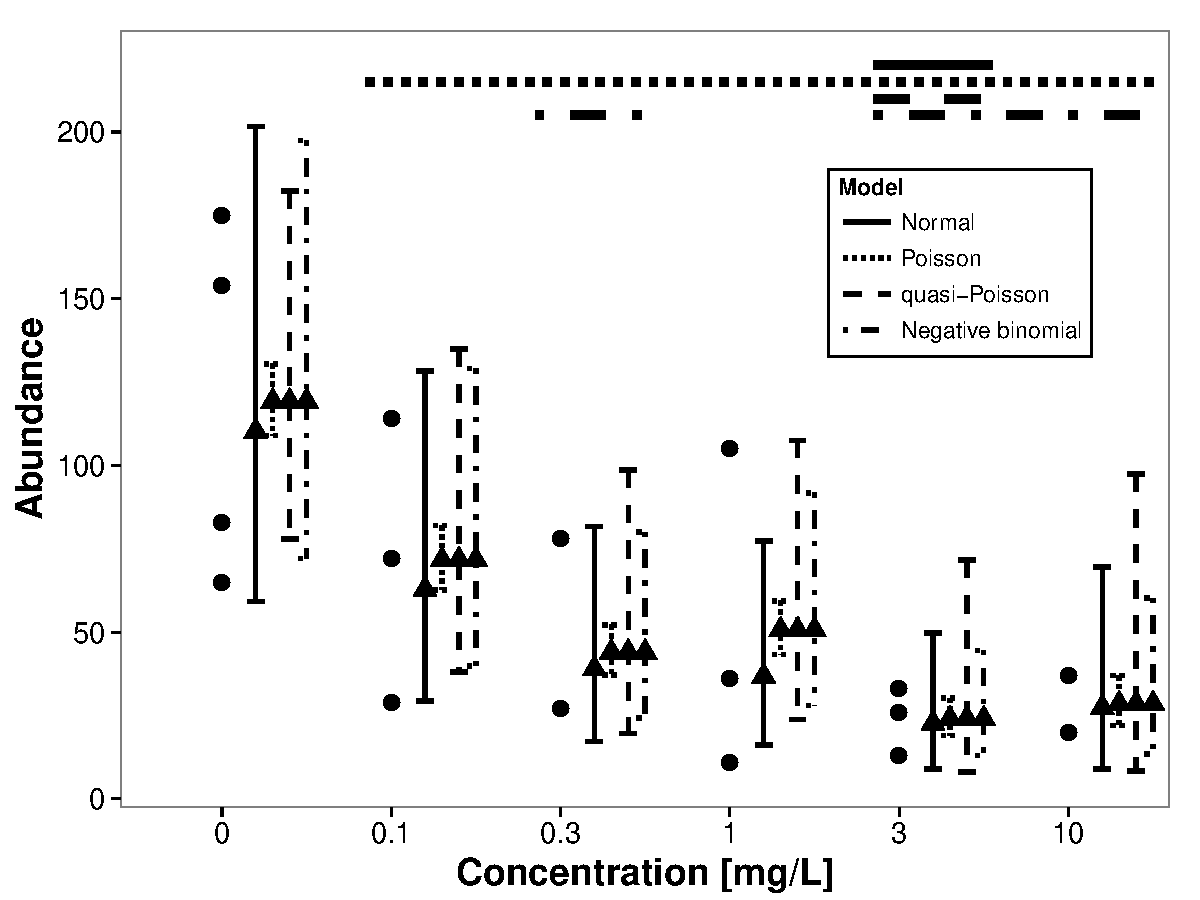
\includegraphics[width = 0.7\textwidth]{example.pdf}
  \caption{Data from \citet{brock_minimum_2015} (boxplots + black points within boxes). 
  Predicted values (triangles) and 95\% Wald Z or t confidence intervals from the fitted models (vertical lines) are given besides the boxplots.
  Horizontal bars above indicate treatments statistically significant different from the control group (Dunnett contrasts).}
  \label{fig:example}
\end{figure}




\subsubsection{Hypothesis testing}
On this data set, we could test different hypotheses like (i) if there is any effect of the treatment or (ii) test single parameters (treatments) to determine the LOEC.
Following general recommendations \citep{bolker_generalized_2009}, we used F-tests for the normal and quasi-Poisson models and Likelihood-Ratio (LR) tests for Poisson and negative binomial models to test if there is any treatment related effect.
To assess the LOEC we used Dunnett contrasts with one-sided Wald t tests (normal and quasi-Poisson models) and one-sided Wald Z tests (Poisson and negative binomial models).


\subsubsection{Results}
The Poisson model showed considerable overdispersion and did not fit the data. 
This leads to underestimated standard errors and confidence intervals and overestimated statistical significance.
Therefore, inferences on the Poisson model are not valid and we do not further discuss its results.
The normal (F = 2.57, p = 0.084) and quasi-Poisson model (F = 2.90, p = 0.061) did not indicate any treatment related effects.
Whereas the LR test of the negative binomial model indicated a treatment related effect (LR = 13.99, p = 0.016).

All methods resulted in similar predicted values, except the normal model predicting always lower abundances (Figure \ref{fig:example}). 
95\% Confidence intervals (CI) where most narrow for the negative binomial model and widest for quasi-Poisson - especially at lower estimated abundances.
Accordingly, the LOECs differed (Normal and quasi-Poisson: 3 mg/L, negative binomial: 0.3 mg/L).

\citet{brock_minimum_2015} assumed normality after data transformation and reported a LOEC of \mbox{0.3 mg/L} for this data.
The reason for this difference may be twofold: \citep{brock_minimum_2015} used a $log(2~y + 1)$ transformation, whereas we used a $log(0.182~y + 1)$ transformation \citep{van_den_brink_impact_2000}.
Moreover, we applied a one-sided Dunnett test, as the toxic response in a mesocosm experiment may be either decreasing or increasing (due to biological interactions).
\citet{brock_minimum_2015} used a one-sided Williams test, which is known to have larger power if the assumptions are met \citep{jaki_statistical_2013}.
This example demonstrates that the choice of the statistical model and procedure has substantial impact on ecotoxicological inferences, especially when sample sizes are low.



\subsection{Binomial data}





\subsubsection{Generalized Linear Models}

We used F-test for the normal and LR test for binomial GLM to determine a general treatment effect.
LOEC was assessed using one-sided Dunnett contrasts.


\subsubsection{Results}
Both methods lead to same ecotoxicological inferences:
The global tests of both methods indicated a effect of NaPCP on larval survival (linear model: F = 13.31, p \textless 0.001; GLM: LR = 64.79, p \textless 0.001).
Moreover, both methods identified the highest concentration (512 \textmu g/L) as LOEC. 

The coefficients of the binomial model are directly interpretable as change in odds ratio:
Compared to the control group, odds in the highest treatment are reduced by a factor of $e^{-3.675} = 0.025$.
Such a direct interpretation of parameters is not possible with the transformed data (Table \ref{tab:ex_bin}).

\begin{table}
\centering
\footnotesize
\caption{Estimated parameters and 95\% Confidence Intervals for the binomial data example. 
Asterisks indicate LOEC as determined using one-sided Dunnett tests.}
\label{tab:ex_bin}
\begin{tabular}{lllll}
\hline
 & \multicolumn{4}{c}{Model} \\ 
Treatment & \multicolumn{2}{c}{LM} & \multicolumn{2}{c}{GLM} \\ 
\cmidrule(lr){2-3} \cmidrule(lr){4-5} 
Control & 1.331 & (1.169, 1.149) & 2.994 & (1.523, 4.366) \\ 
32 \textmu g/L  & -0.147 & (-0.376, 0.081) & -1.210 & (2.876, 0.456) \\ 
64 \textmu g/L  & 0.041 & (-0.188, 0.269) & 0.719 & (-1.723, 3.161) \\ 
128 \textmu g/L  & -0.076 & (-0.305, 0.152) & -0.747 & (-2.505, 1.010) \\ 
256 \textmu g/L & -0.221 & (-0.450, 0.007) & -1.708 & (-3.312, -0.104) \\ 
512 \textmu g/L  & -0.727 & (-0.956, -0.499)$*$ & -3.675 & (-5.244, -2.107)$*$ \\ 
\hline
\end{tabular}
\end{table}


%% --------------------------------
\section{Simulations}
\label{sec:sim}
We used simulations to compare the methods described above to analyse count and binomial data.
Methods were compared in terms of Type I error (maintain a significance level of 0.05 when there is no effect) and power (detect an effect when it is present). 
We fitted the models and tested hypotheses on the simulated data as described in the motivating examples.

All simulations were done in R (Version 3.1.2) \citep{r_core_team_r:_2014} on a 64-bit Linux machine with 8 GB and 2.2 GHz.
Source code for the simulations is available online at \url{https://github.com/EDiLD/usetheglm}.

\subsection{Count data}
 

\subsubsection{Results}
At small sample sizes (n = {3, 6}) and low abundances ($\mu_C$ = {2, 4}) many of the negative binomial models ($GLM_{nb}$ and $GLM_{pb}$) did not converge to a solution (convergence rate \textless 80\% of the simulations, Supplement 1). 
For this simulation design (reduction in abundance by 50\%) a sample size of n = 9 was needed to achieve a power greater than 80\%.
$GLM_{nb}$ showed an increased Type I error at low sample sizes. 
However, this decreased with increasing sample sizes (Figure \ref{fig:p_glob_c}, bottom).
Using parametric bootstrap ($GLM_{pb}$) resulted in an appropriate Type 1 error level for the negative binomial model.
$LM$, $GLM_{qp}$ maintained also an appropriate Type I error.
The Kruskal-Wallis test showed the least power, with low Type I error at small sample sizes. 
All GLM showed greater power than $LM$ or the Kruskal test. 
$GLM_{qp}$ showed up to 17\% greater power compared to $LM$.

\begin{figure}
  \centering
  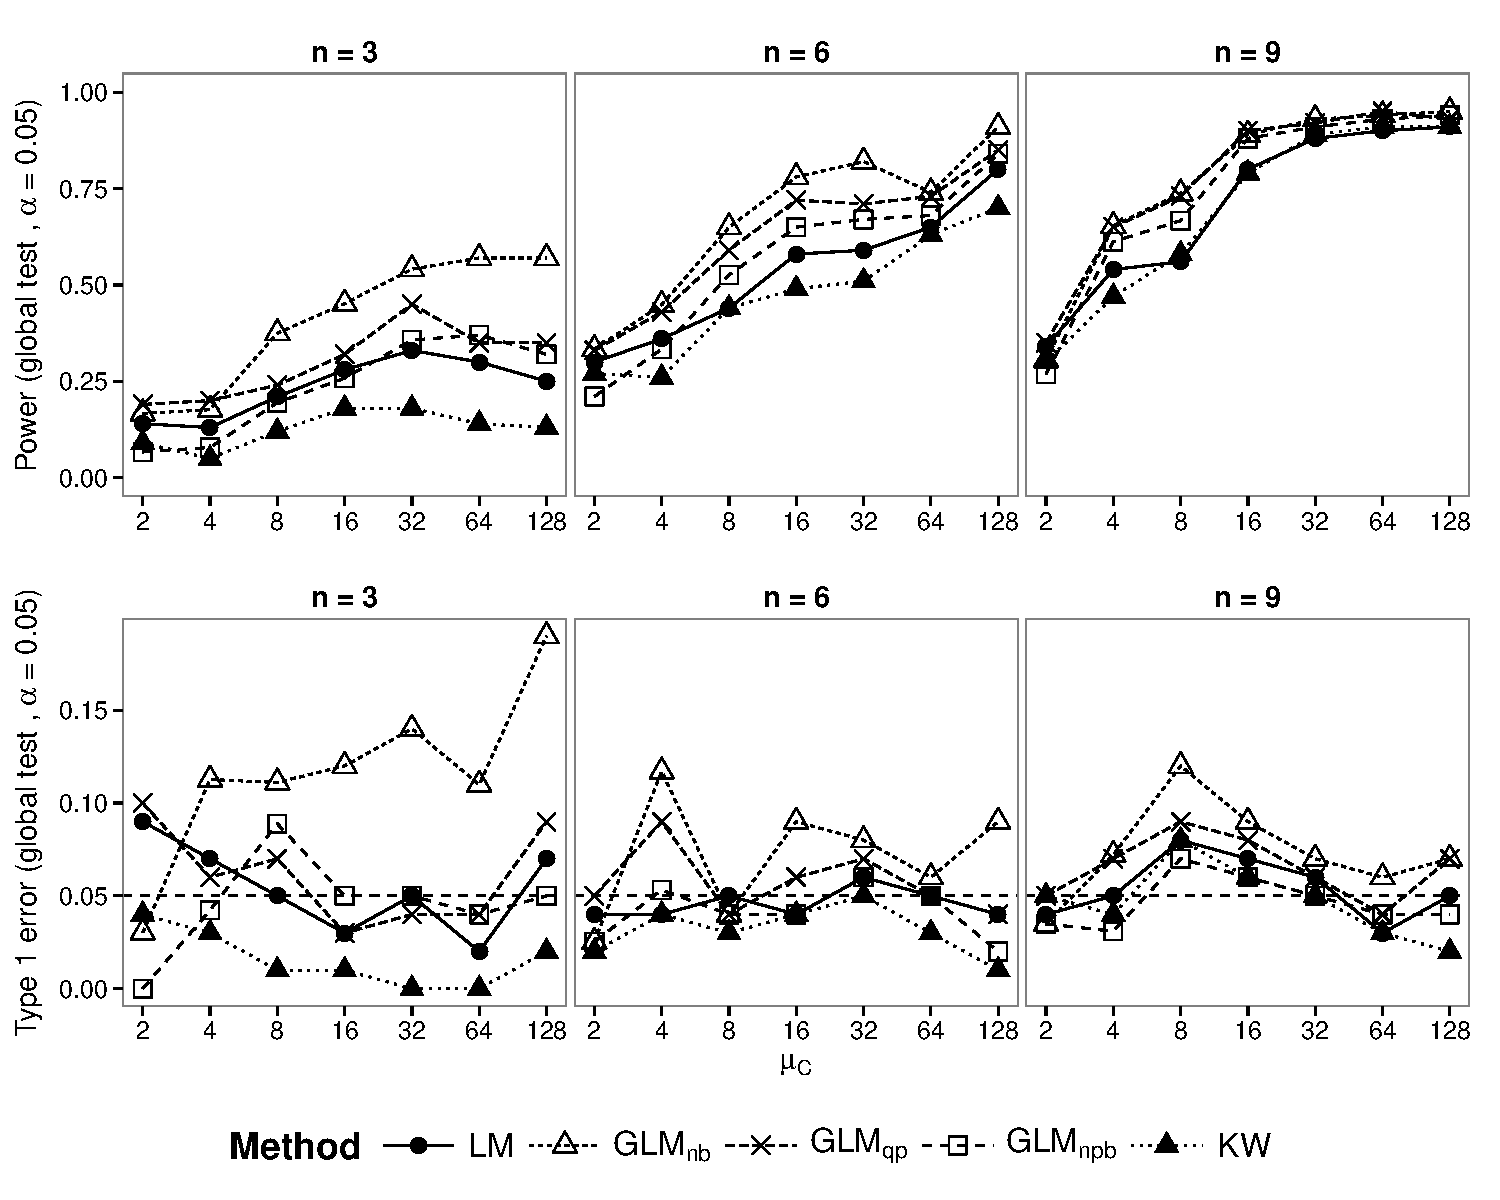
\includegraphics[width = 0.8\textwidth]{p_glob_c.pdf}
  \caption{Simulation results for count data. Power (top) and Type I error (bottom) for the test of a treatment effect. Compared methods were: Linear model after log (Ax + 1) transformation (lm), negative binomial GLM with LRT (glm\_nb), negative binomial GLM with parametric boostrap (glm\_pb), quasi-Poisson GLM (glm\_qp) and Kruskal-Wallis test on untransformed data (np).
  For n = 3 and $\mu_C$ = {2, 4} less then 80\% of glm\_nb and glm\_pb models did converge.}
  \label{fig:p_glob_c}
\end{figure}

The inferences on LOEC generally showed less power.
For $LM$ this reduction was up to 35\% (Figures \ref{fig:p_glob_c} and \ref{fig:p_loec_c}).
At low sample sizes $GLM_{nb}$ showed an increased Type 1 error and the pairwise Wilcoxon Test had no power at all to detect the correct LOEC.
$GLM_{qp}$ and $LM$ yielded comparable Type 1 errors, with $GLM_{qp}$ having up to 11\% greater power (Figure \ref{fig:p_loec_c}, top).

\begin{figure}
  \centering
  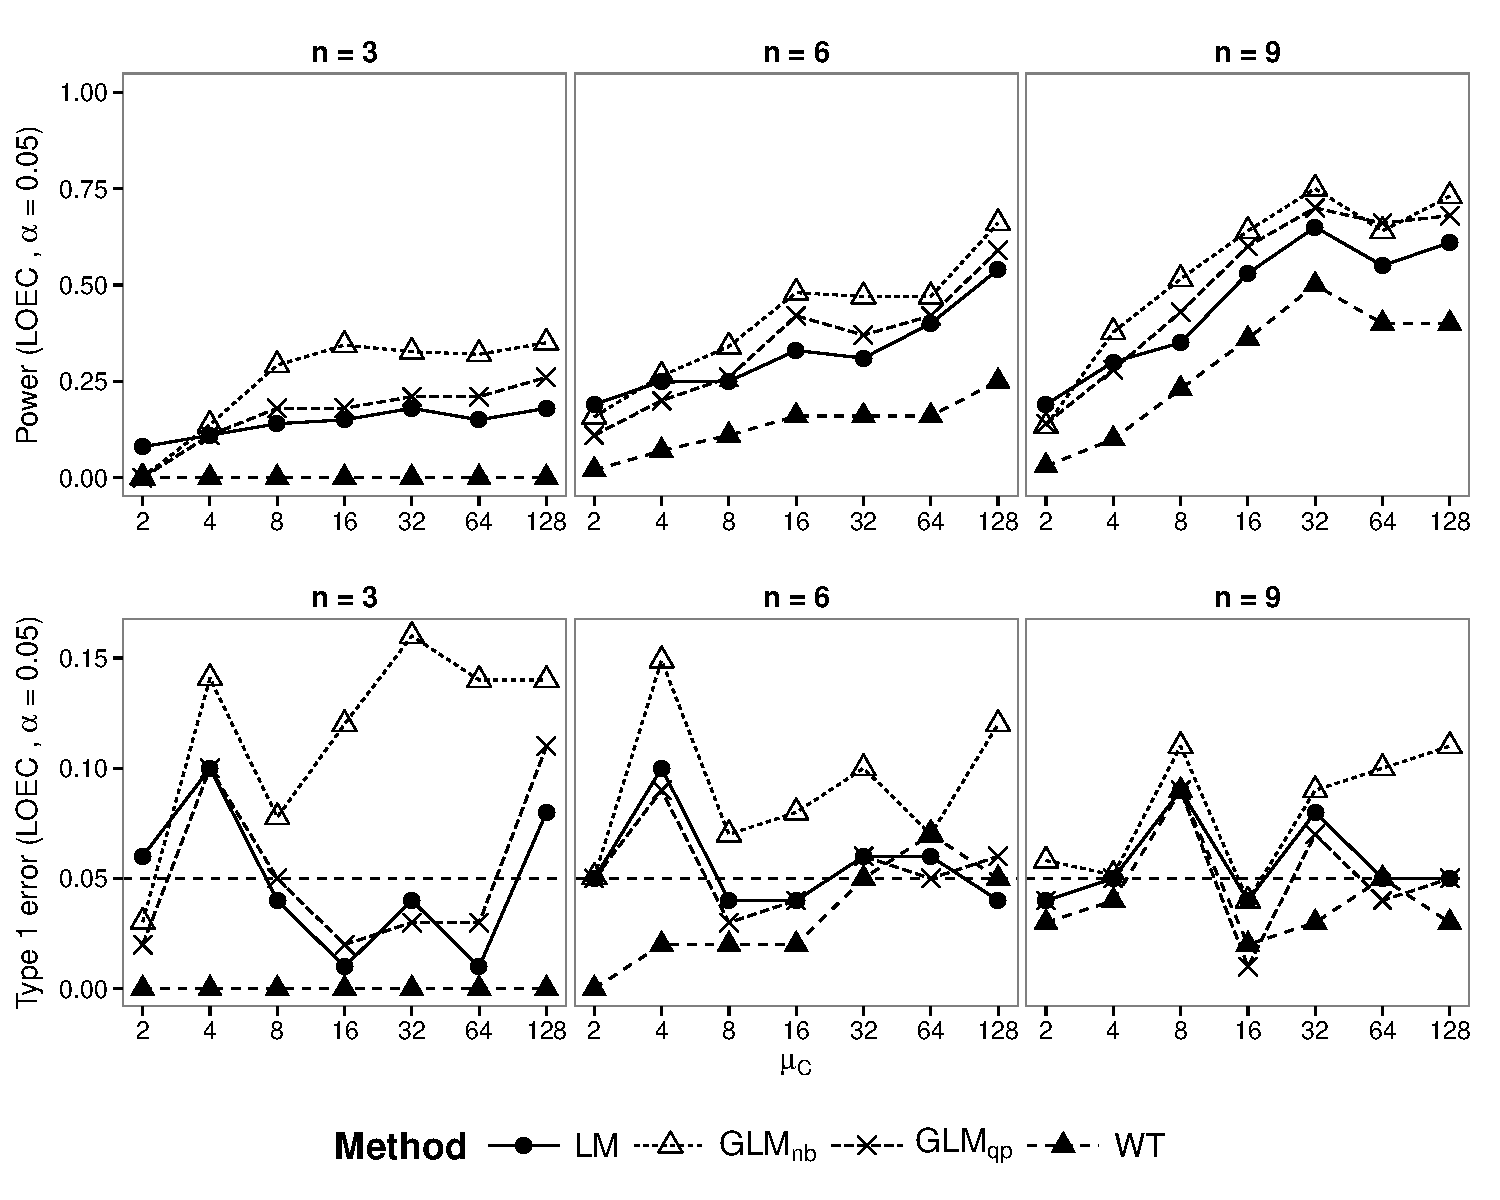
\includegraphics[width = 0.8\textwidth]{p_loec_c.pdf}
  \caption{Simulation results for count data. Power (top) and Type I error (bottom) for determination of LOEC. Compared methods were: Linear model after log (Ax + 1) transformation (lm), negative binomial GLM with LRT (glm\_nb), negative binomial GLM with parametric boostrap (glm\_pb), quasi-Poisson GLM (glm\_qp) and pairwise Wilcoxon test on untransformed data (np). For n = 3 and $\mu_C$ = {2, 4} less then 80\% of glm\_nb and glm\_pb models did converge.}
  \label{fig:p_loec_c}
\end{figure}



\subsection{Binomial data}



\subsubsection{Results}
Binomial GLM showed the greatest power for testing the treatment effect, while maintaining an appropriate Type I error level.
This was especially apparent at low sample sizes (n = 3), with up to 24\% higher power.
Kruskal-Wallis test had the lowest power and a low Type I error rate.
However, the difference between methods quickly vanished with increasing samples sizes (Figure \ref{fig:p_glob_p}).

\begin{figure}
  \centering
  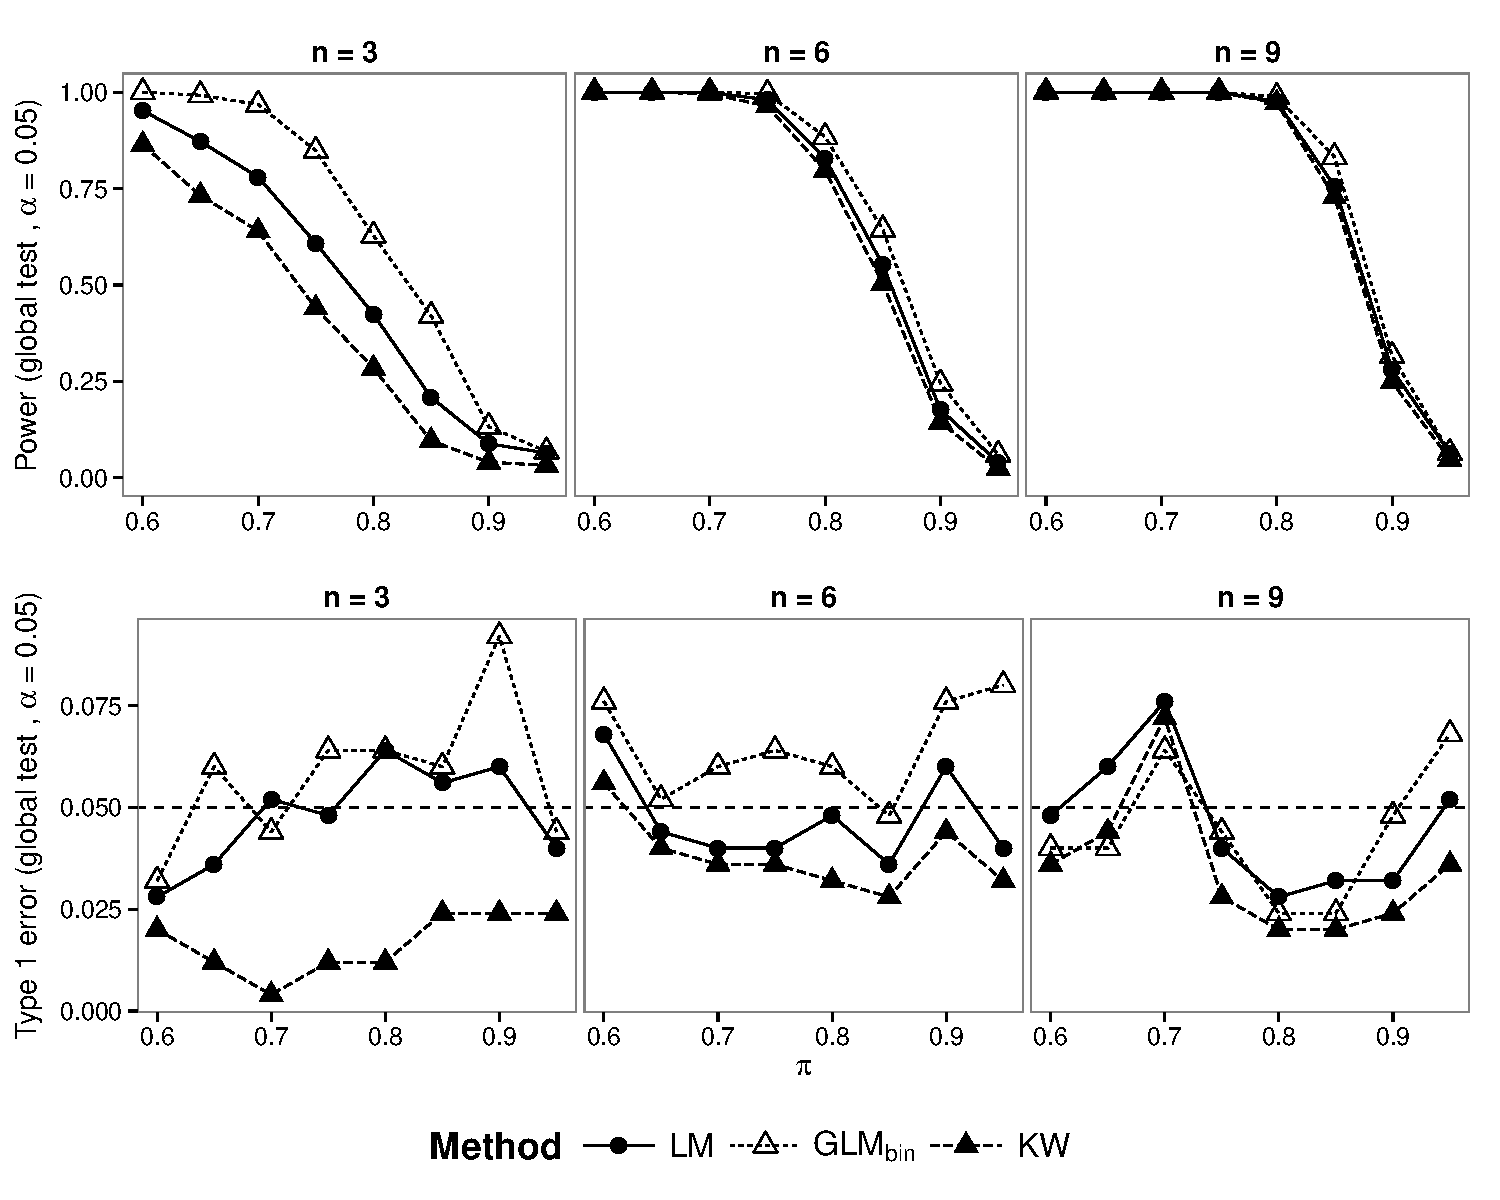
\includegraphics[width = 0.8\textwidth]{p_glob_p.pdf}
  \caption{Simulation results for binomial data. Power (top) and Type I error (bottom) for the test of a treatment effect. Compared methods were: Linear model after arcsine square root transformation (lm), binomial GLM with LRT (glm) and Kruskal-Wallis test on untransformed data (np).}
  \label{fig:p_glob_p}
\end{figure}

Inference on LOEC was not as powerful as inference on the general treatment effect.
Contrary to the global test, $LM$ showed the highest power for small sample sizes, while maintaining a Type 1 error level of 0.05.
$GLM$ had less power and showed a lower Type 1 error rate, especially with decreasing effect size.
The pairwise Wilcoxon test had no power at all for n = 3 and showed less power in the other simulation runs.
Differences in power to detect a LOEC was only apparent at n = 3 and vanished quickly with increasing sample sizes (Figure \ref{fig:p_loec_p}). 

\begin{figure}
  \centering
  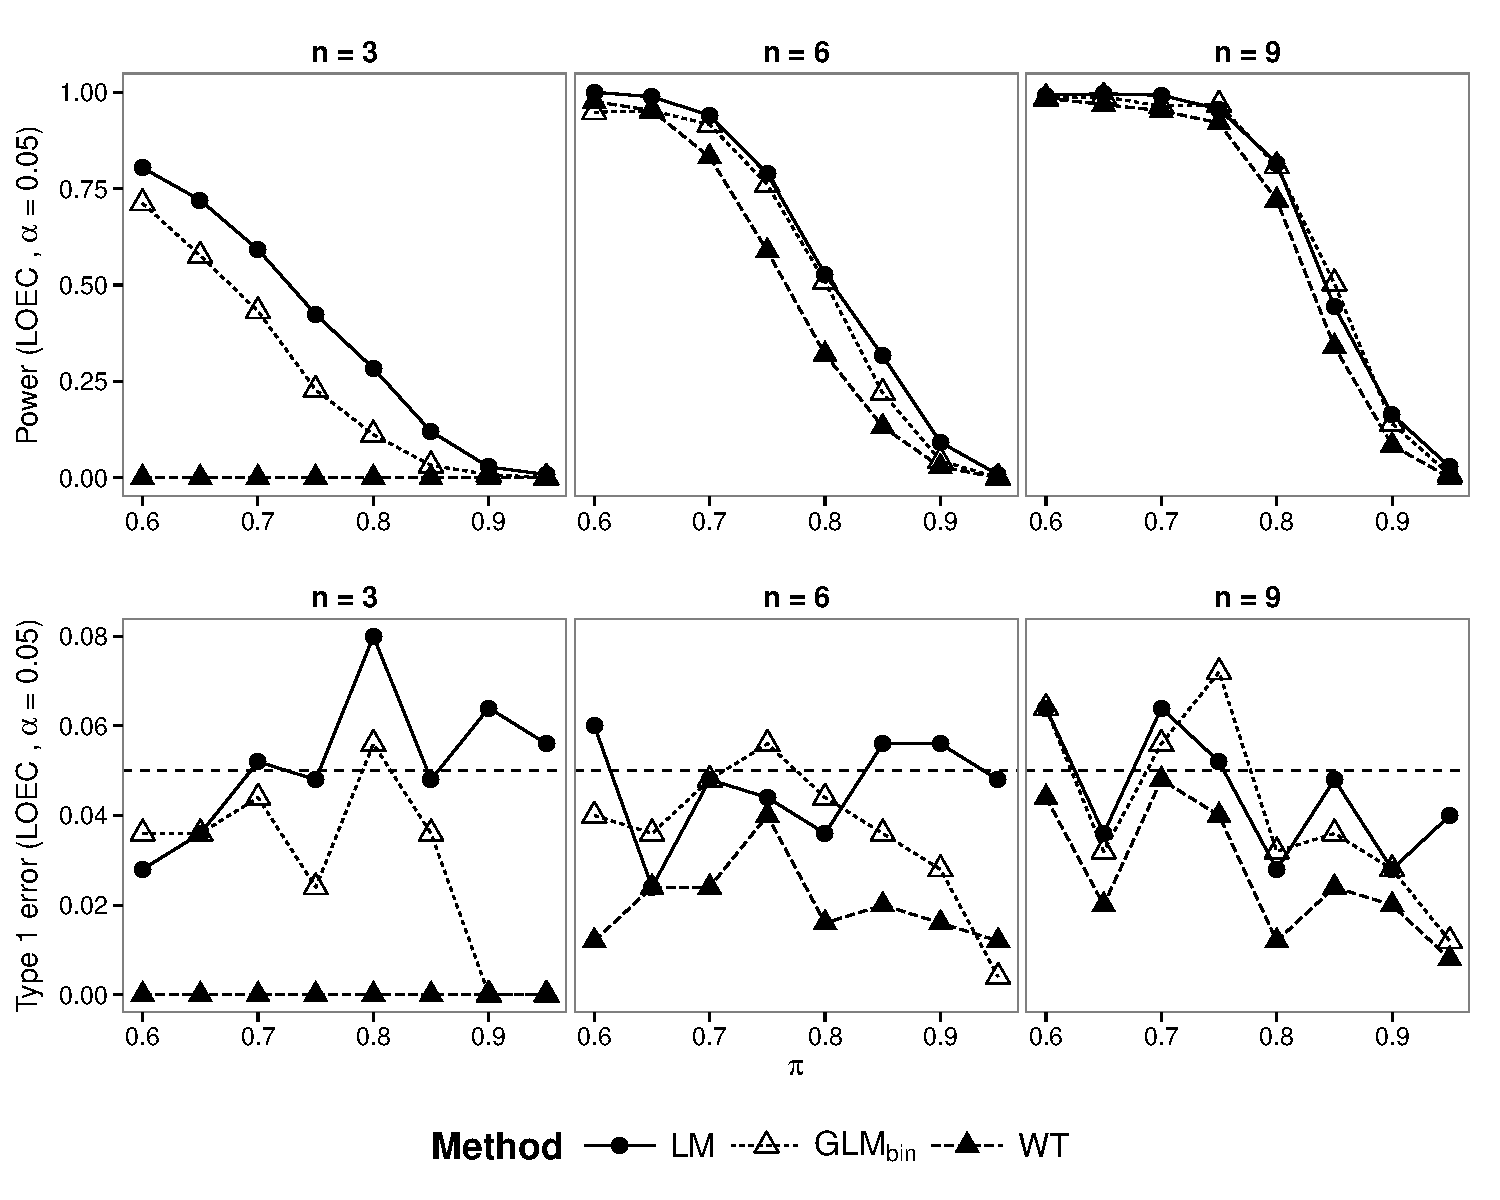
\includegraphics[width = 0.8\textwidth]{p_loec_p.pdf}
  \caption{Simulation results for binomial data. Power (top) and Type I error (bottom) for determination of LOEC. Compared methods were: Linear model after arcsine square root transformation (lm), binomial GLM with LRT (glm) and a pairwise Wilcoxon test on untransformed data (np).}
  \label{fig:p_loec_p}
\end{figure}



%% --------------------------------
\section{Discussion}
\label{sec:disc}
%% --- general low power
Ecotoxicological experiments are often planned with small sample sizes due to practical constraints. 
For example, extremely low samples sizes (n \textless 5) are common in cases \citep{sanderson_pesticide_2002,szocs_analysing_2015}.
Statistical power is crucial for the determination of LOEC/NOEC values.
Although the use of LOEC/NOEC has been heavily criticized in the past \citep{landis_well_2011},  they are still regularly used in ecotoxicology \citep{jager_bad_2012}.
Especially in mesocosm studies NOEC calculations are used in the majority of mesocosm experiments \citep{brock_minimum_2015,efsa_ppr_guidance_2013}.
To counteract the problems with low power \citet{brock_minimum_2015} proposed to take the Minimum Detectable Difference (MDD), a method to assess statistical power \emph{a posteriori}, for inference into account.
Our results suggest that power in common mesocosm experiments is low.
For common samples sizes and a reduction in abundance of 50\% we found an unacceptably low power to detect any treatment related effect (\textless 50\% for methods with appropriate Type 1 error, Figure \ref{fig:p_glob_c}).
Additionally, \citet{ohara_not_2010} showed that using a log transformation gave unreliable and biased parameter estimates.
Statistical power to detect the correct LOEC was even worse, with power less than 30\%.
This suggests that NOECs reported from mesocosm experiments should be interpreted with caution and underpins the critics on NOEC.
\emph{A priory} power analyses can be performed easily using simulations, even for complex experimental designs \citep{johnson_power_2014}, and might help to design, interpret and evaluate ecotoxicological studies.

Moreover, \citet{brock_minimum_2015} proposed that statistical power of mesocosm experiments can be increased by reducing sampling variability by better sampling and quantification methods. 
But they also caution to avoid depleting populations by increasing sampling efficiency.
As we showed, using appropriate statistical methods (like GLMs) can enhance the power at no extra costs.

%% --- Non-parametric
It has been advocated that in the typical case of small sample sizes (n \textless 20) and non-normal data, non-parametric tests perform better than parametric tests assuming normality \citep{wang_making_2011}.
In contrast, our results showed that the often applied Kruskal test and pairwise Wilcoxon test have equal or less power compared to tests assuming normality after data transformation.
Moreover, GLMs always performed better than non-parametric tests. 
However, there might be more powerful non-parametric tests available \citep{konietschke_rank-based_2012} which we did not investigate.
Non-parametric statistics are focused on testing but not on estimation of effects.
Additionally to testing, GLMs allow the estimation and interpretation of effects that might not be statistically significant, but ecologically relevant.
Therefore, we do not advise to use non-parametric tests for non-normal data but GLMs instead.

%% ---- Problems GLM
At small sample sizes and low abundance a significant amount of negative binomial models did not converge.
We used an iterative algorithm to fit these models \citep{venables_modern_2002} and other methods assessing directly the likelihood may perform better.
Moreover, the Likelihood-Ratio test gave increased Type-I error for these models.
It is well known that the LR statistic is unreliable for small sample sizes \citep{bolker_generalized_2009,wilks_large-sample_1938} and we found that parametric bootstrap provides a valuable alternative in such situations.
At small samples sizes and / or low abundances it might be hard to decide which mean-variance relationship fits best.
The quasi-Poisson models assumes a simpler, linear mean-variance relationship, which might explain why it performed best for our simulated data sets. 


%% --- binomial data
Binomial data is often collected in lab trials, where increasing sample size is easier to accomplish. 
We found notable differences in power to detect a treatment effect up to a sample size of 9.
Similarly, \citet{warton_arcsine_2011} also found that GLM have higher power than arcsine transformed linear models.
However, for deriving LOECs the normal model performed better at low sample sizes. At samples sizes greater than three we found no power differences for detecting the correct LOEC.
The interpretation of binomial GLMs is much simpler than for the arcsine transformed data.
Their power is is equal or even higher at sample sizes greater then three. 
Therefore, we recommend to use binomial GLM instead of the arcsine transformation.

%% ---- Guideline GLMs
In the introduction we pointed out that there is little advice how to choose from the plenty of possible transformations.
How do GLMs simplify this problem?
First of all, the distribution modelled should be chosen to give a statistically sound model.
Proportions are bounded between 0 and 1 and could be modelled using a binomial distribution.
Counts are positive discrete values and should be modelled with a discrete distribution.
In a factorial design the mean-variance relationship can be easily checked with diagnostic plots.
Moreover, it should be checked for overdispersion. 
Standard error will be underestimated and significance overestimated, if not accounted for (Figure \ref{fig:example}).
The model selection process can be guided by the data and diagnostic plots. Therefore, it is much more sound than choosing between transformations.


%% --- Multivariate + GLMM -------
Although our simulations covered only simple experimental designs, these findings may also extend to more complex designs. 
Nested or repeated designs with non-normal data could be analysed using Generalized Linear Mixed Models (GLMM) and may have advantages with respect to power \citep{stroup_rethinking_2014}.
For community analyses \emph{GLM for multivariate data} have been proposed as alternative to Principal Response Curves (PRC) and yielded to similar inferences, but better indication of responsive taxa \citep{warton_distance-based_2012,szocs_analysing_2015}.



%% --------------------------------
\section{Conclusions}
\label{sec:concl}
Statistical hypothesis tests are commonly used in environmental risk assessments  to make inferences on pesticide effects.
The choice how we treat, model and test the data can have massive impacts on the conclusions we draw from experiments especially at low sample sizes.
We showed for two common data types in ecotoxicology, that using appropriate models resulted in higher statistical power than trying to meet the assumptions of normality and variance homogeneity using transformations. 
Therefore, we cannot recommend the current practice to either transform the data or use non-parametric approaches if data is not normally distributed.
We recommend to use models that fit to the data. 
GLMs should become a standard method in ecotoxicology and guidelines need to be updated accordingly.



%% --------------------------------
\bibliography{references}
\bibliographystyle{apalike}

\end{document}
